
\section{Proportional Symbol Mapping}
\label{sec-1}
\label{sec:bubble}
\subsection{Introduction}
\label{sec-1-1}
The proportional symbol technique uses symbols of different sizes
to represent data associated with areas or point locations, with
circles being the most frequently used geometric symbol. The data
and the size of symbols can be related through different types of
scaling: mathematical scaling sizes areas of point symbols in
direct proportion to the data; perceptual scaling corrects the
mathematical scaling to account for visual understimation of
larger symbols; and range grading, where data are grouped, and each
class is represented with a single symbol size. 

In this chapter we display data from a grid of sensors belonging to
the Integrated Air Quality system of the Madrid City Council (Section
\ref{sec:airQualityData}) with circles as the proportional symbol, and
range grading as the scaling method. The objective when using range
grading is to discriminate between classes instead of estimating an
exact value from a perceived symbol size. However, because human
perception of symbol size is limited, it is always recommended to
add a second perception channel to improve the discrimination
task. Colors from a sequential palette will complement symbol size to
encode the groups.

\subsection{Proportional Symbol with \texttt{spplot}}
\label{sec-1-2}
The \texttt{NO2sp} \texttt{SpatialPointsDataFrame} can be easily displayed
with the \texttt{spplot} method provided by the \texttt{sp} package, based on
\texttt{xyplot} from the \texttt{lattice} package. Both color and size can be
combined in a unique graphical output because \texttt{spplot} accepts
both of them (Figure \ref{fig:airMadrid_spplot}). I define a
sequential palette whose colors denote the value of the variable
(green for lower values of the contaminant, brown for intermediate
values, and black for highest values).

\lstset{language=R,numbers=none}
\begin{lstlisting}
library(sp)

load('data/NO2sp.RData')
\end{lstlisting}

\lstset{language=R,numbers=none}
\begin{lstlisting}
airPal <- colorRampPalette(c('springgreen1', 'sienna3', 'gray5'))(5)

spplot(NO2sp["mean"], col.regions=airPal, cex=sqrt(1:5),
       edge.col='black', scales=list(draw=TRUE),
       key.space='right')
\end{lstlisting}

\begin{figure}[htb]
\centering
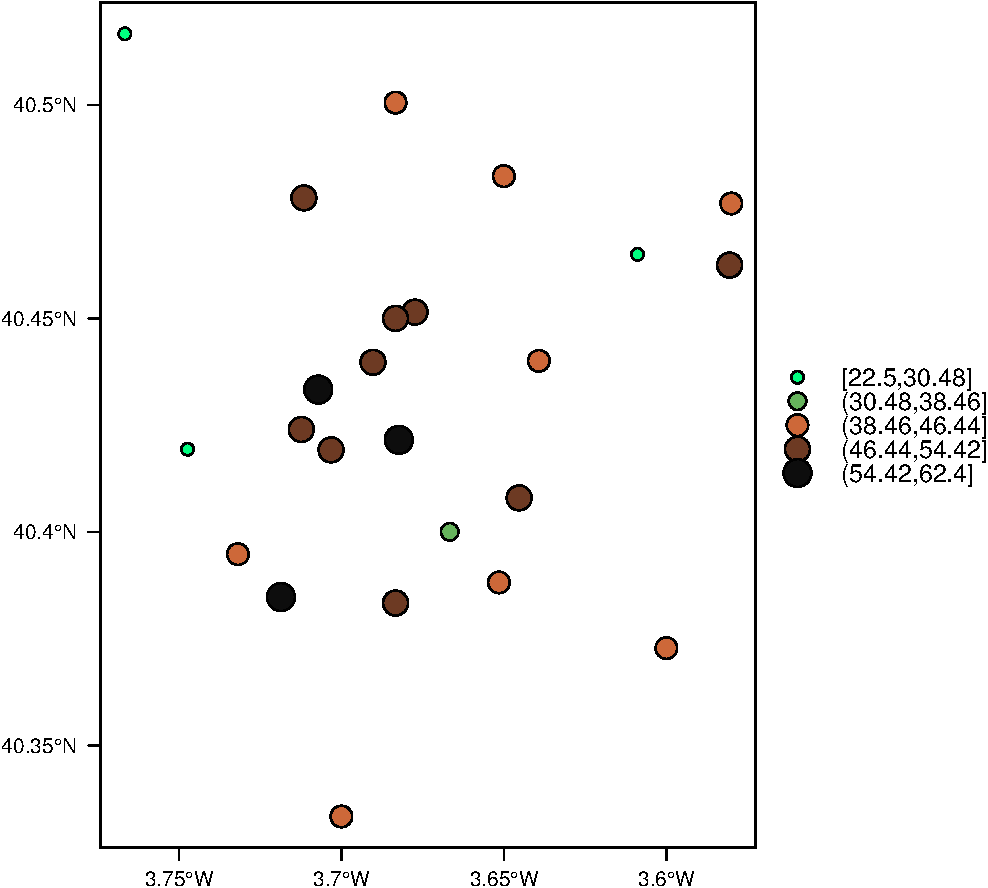
\includegraphics[width=.9\linewidth]{figs/airMadrid_spplot.pdf}
\caption{\label{fig:airMadrid_spplot}Annual average of $NO_2$ measurements in Madrid. Values are shown with different symbol sizes and  colors for each class with the \texttt{spplot} function.}
\end{figure}

The \texttt{ggplot2} version of this code needs to transform the
\texttt{SpatialPointsDataFrame} to a conventional \texttt{data.frame} (which
will contain two columns with latitude and longitude values).
\lstset{language=R,numbers=none}
\begin{lstlisting}
NO2df <- data.frame(NO2sp)
NO2df$Mean <- cut(NO2sp$mean, 5)

ggplot(data=NO2df, aes(long, lat, size=Mean, fill=Mean)) +
    geom_point(pch=21, col='black') + theme_bw() +
    scale_fill_manual(values=airPal)
\end{lstlisting}
\subsection{Optimal Classification and Sizes to Improve Discrimination}
\label{sec-1-3}
Two main improvements can be added to Figure
\ref{fig:airMadrid_spplot}:

\begin{itemize}
\item Define classes dependent on the data structure (instead of the
uniform distribution assumed with \texttt{cut}). A suitable approach is
the \texttt{classInterval} function of the \texttt{classInt} package, which
implements the Fisher-Jenks optimal classification
algorithm.
\end{itemize}

\index{Packages!classInt@\texttt{classInt}}
\index{classIntervals@\texttt{classIntervals}}
\index{findCols@\texttt{findCols}}
\index{findColours@\texttt{findColours}}

\lstset{language=R,numbers=none}
\begin{lstlisting}
library(classInt)
## The number of classes is chosen between the Sturges and the
## Scott rules.
nClasses <- 5
intervals <- classIntervals(NO2sp$mean, n=nClasses, style='fisher')
## Number of classes is not always the same as the proposed number
nClasses <- length(intervals$brks) - 1
\end{lstlisting}

\lstset{language=R,numbers=none}
\begin{lstlisting}
op <- options(digits=4)
tab <- print(intervals)
options(op)
\end{lstlisting}

\begin{itemize}
\item Encode each group with a symbol size (circle area) such that visual
discrimination among classes is enhanced. The next code uses the set
of radii proposed in \cite{Dent.Torguson.ea2008} (Figure
\ref{fig:dent}). This set of circle sizes is derived from studies by Meihoefer \cite{Meihoefer1969}. He derived a set of ten
circle sizes that were easily and consistently discriminated by his
subjects. The alternative proposed by Dent et al. improves the
discrimination between some of the circles.
\end{itemize}

\lstset{language=R,numbers=none}
\begin{lstlisting}
## Complete Dent set of circle radii (mm)
dent <- c(0.64, 1.14, 1.65, 2.79, 4.32, 6.22, 9.65, 12.95, 15.11)
## Subset for our dataset
dentAQ <- dent[seq_len(nClasses)]
## Link Size and Class: findCols returns the class number of each
## point; cex is the vector of sizes for each data point
idx <- findCols(intervals)
cexNO2 <- dentAQ[idx]
\end{lstlisting}

\begin{figure}[htb]
\centering
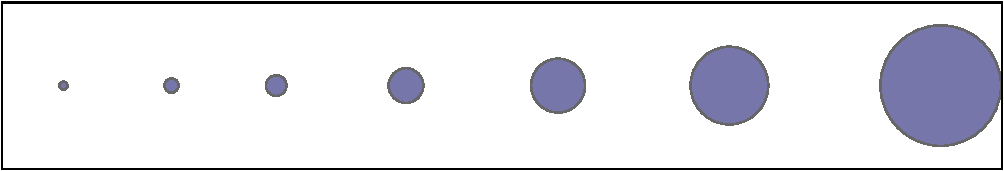
\includegraphics[width=.9\linewidth]{figs/dent.pdf}
\caption{\label{fig:dent}Symbol sizes proposed by Borden Dent.}
\end{figure}

These two enhancements are included in Figure
\ref{fig:airMadrid_classes}, which displays the categorical variable
\texttt{classNO2} (instead of \texttt{mean}) whose levels are the intervals
previously computed with \texttt{classIntervals}. In addition, this
figure includes an improved legend.

\lstset{language=R,numbers=none}
\begin{lstlisting}
NO2sp$classNO2 <- factor(names(tab)[idx])
\end{lstlisting}

\lstset{language=R,numbers=none}
\begin{lstlisting}
## ggplot2 version
NO2df <- data.frame(NO2sp)

ggplot(data=NO2df, aes(long, lat, size=classNO2, fill=classNO2)) +
    geom_point(pch=21, col='black') + theme_bw() +
    scale_fill_manual(values=airPal) +
    scale_size_manual(values=dentAQ*2)
\end{lstlisting}

\lstset{language=R,numbers=none}
\begin{lstlisting}
## spplot version

## Definition of an improved key with title and background
NO2key <- list(x=0.98, y=0.02, corner=c(1, 0),
	      title=expression(NO[2]~~(paste(mu, plain(g))/m^3)),
	      cex.title=.75, cex=0.7,
	      background='gray92')

pNO2 <- spplot(NO2sp["classNO2"],
	       col.regions=airPal,  cex=dentAQ,
	       edge.col='black',
	       scales=list(draw=TRUE),
	       key.space=NO2key)
pNO2
\end{lstlisting}

\begin{figure}[htb]
\centering
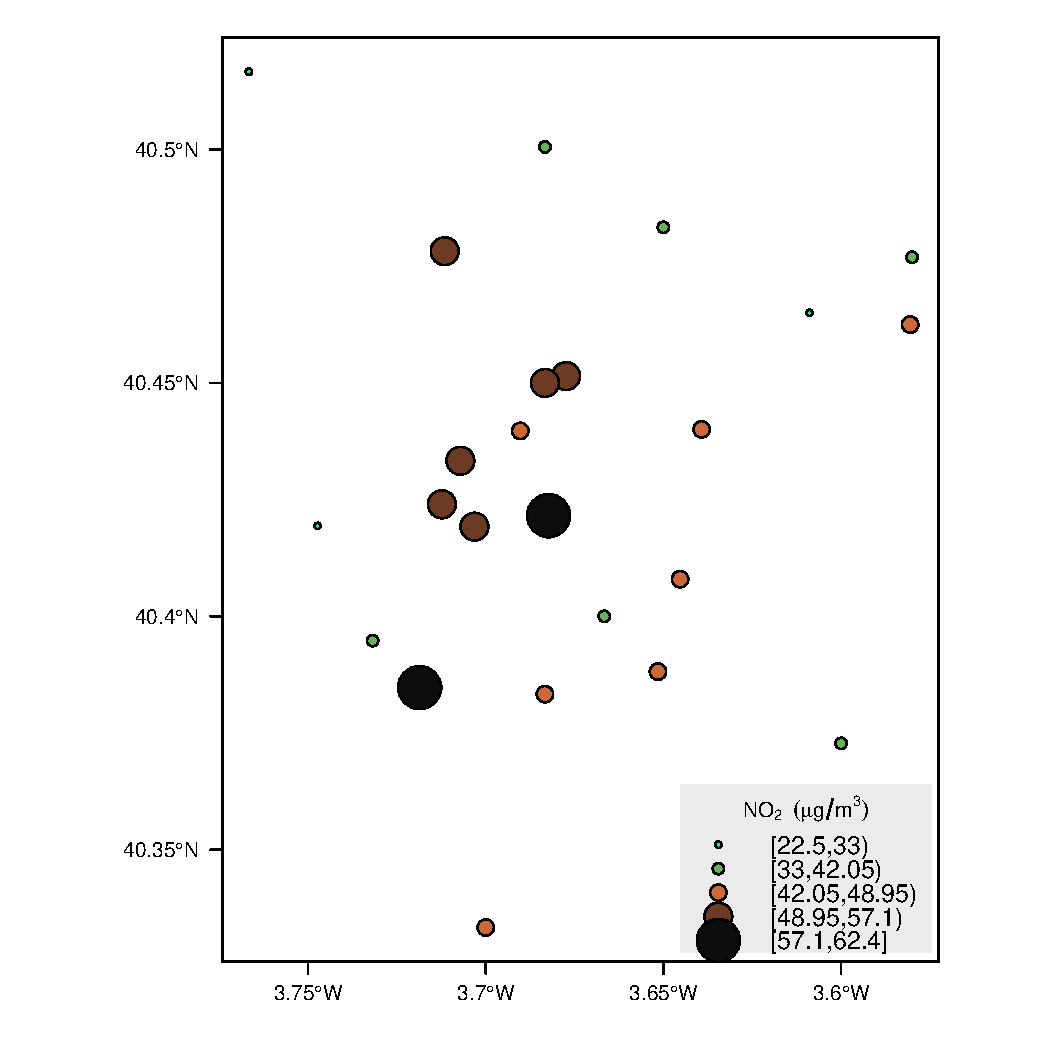
\includegraphics[width=.9\linewidth]{figs/airMadrid_classes.pdf}
\caption{\label{fig:airMadrid_classes}Annual average of $NO_2$ measurements in Madrid.}
\end{figure}
\subsection{Spatial Context with Underlying Layers and Labels}
\label{sec-1-4}
The spatial distribution of the stations is better understood if
we add underlying layers with information about the spatial
context. 

\subsubsection{Static Image}
\label{sec-1-4-1}
A suitable method is to download data from a provider such as Google
Maps\textsuperscript{\texttrademark} or OpenStreetMap and transform it adequately. There are several
packages that provide an interface to query several map servers. On
one hand, \texttt{RGoogleMaps}, \texttt{OpenStreetMaps}, and \texttt{ggmap} provide raster
images from static maps obtained from Google Maps, Stamen,
OpenStreetMap, etc.; on the other hand, \texttt{osmar} is able to access
OpenStreetMap data and convert it into classes provided by existing R
packages (mainly \texttt{sp} and \texttt{igraph0} objects).

Among these options, I have chosen the Stamen watercolor maps
available through the \texttt{ggmap} \cite{Kahle.Wickham2013} and
\texttt{OpenStreetMaps} packages \cite{Fellows.Stotz2013}. It is worth noting
that these map tiles are published by Stamen Design under a Creative
Commons licence CC BY-3.0 (Attribution). They produce these maps with
data by OpenStreetMap also published under a Creative Commons licence
BY-SA (Attribution - ShareAlike).

\index{Packages!ggmap@\texttt{ggmap}}
\index{Packages!OpenStreetMap@\texttt{OpenStreetMap}}

\lstset{language=R,numbers=none}
\begin{lstlisting}
madridBox <- bbox(NO2sp)

## ggmap solution
library(ggmap)
madridGG <- get_map(c(madridBox), maptype='watercolor', source='stamen')
\end{lstlisting}

\lstset{language=R,numbers=none}
\begin{lstlisting}
## OpenStreetMap solution
library(OpenStreetMap)
ul <- madridBox[c(4, 1)]
lr <- madridBox[c(2, 3)]
madridOM <- openmap(ul, lr, type='stamen-watercolor')
madridOM <- openproj(madridOM)
\end{lstlisting}

\lstset{language=R,numbers=none}
\begin{lstlisting}
NO2df <- data.frame(NO2sp)

## ggmap
ggmap(madridGG) +
    geom_point(data=NO2df,
	       aes(long, lat, size=classNO2, fill=classNO2),
	       pch=21, col='black') +
       scale_fill_manual(values=airPal) +
       scale_size_manual(values=dentAQ*2)

##OpenStreetMap
autoplot(madridOM) + 
    geom_point(data=NO2df,
	       aes(long, lat, size=classNO2, fill=classNO2),
	       pch=21, col='black') +
    scale_fill_manual(values=airPal) +
    scale_size_manual(values=dentAQ*2)
\end{lstlisting}

Although \texttt{ggmap} is designed to work with the \texttt{ggplot2} package, the
result of \texttt{get\_map} is only a \texttt{raster} object with
attributes. Therefore, it can be easily displayed with \texttt{grid.raster}
as an underlying layer of the previous \texttt{spplot} result (Figure
\ref{fig:airMadrid_stamen}).

\lstset{language=R,numbers=none}
\begin{lstlisting}
## the 'bb' attribute stores the bounding box of the get_map result
bbMap <- attr(madridGG, 'bb')
## This information is needed to resize the image with grid.raster
height <- with(bbMap, ur.lat - ll.lat)
width <- with(bbMap, ur.lon - ll.lon)

pNO2 + layer(grid.raster(madridGG,
			  width=width, height=height,
			  default.units='native'),
	     under=TRUE)
\end{lstlisting}

\begin{figure}[htb]
\centering
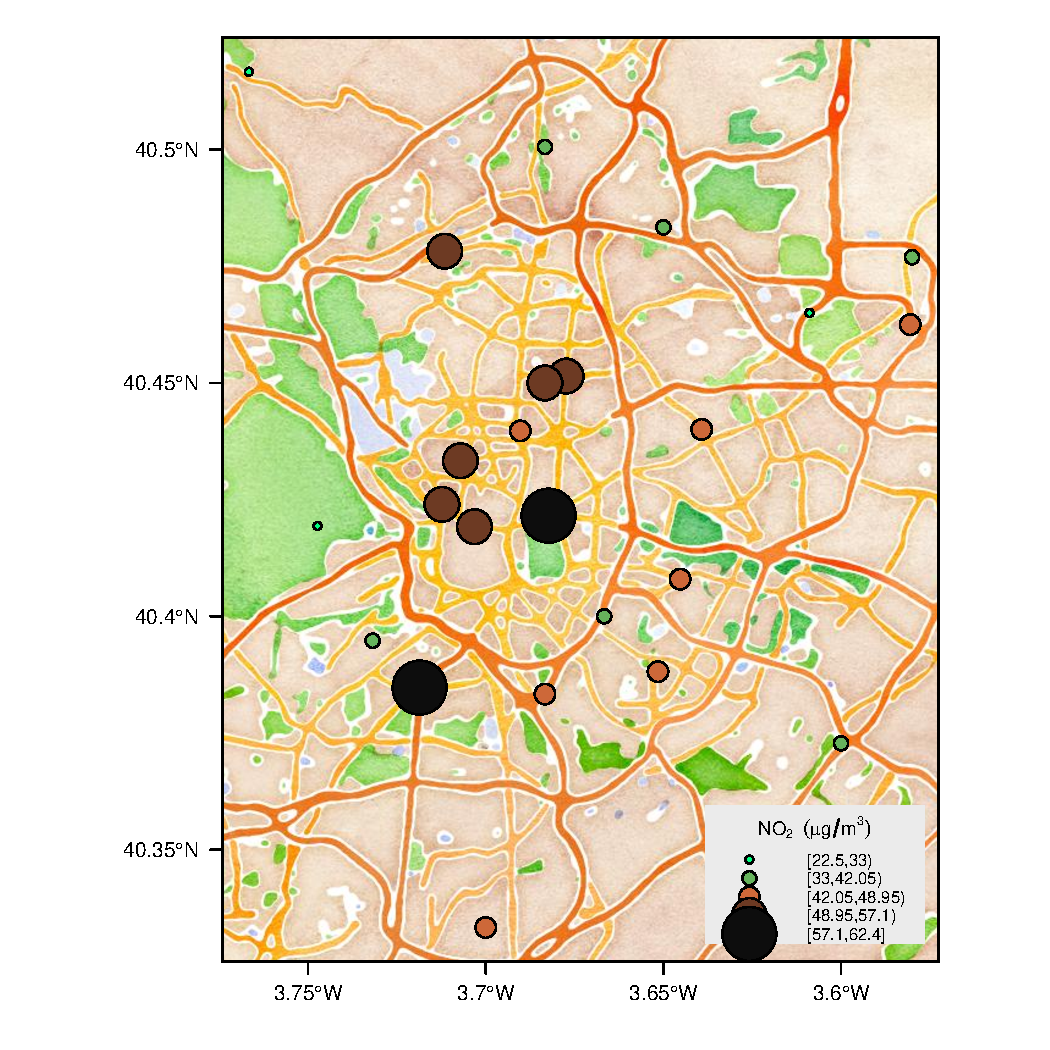
\includegraphics[width=.9\linewidth]{figs/airMadrid_stamen.pdf}
\caption{\label{fig:airMadrid_stamen}Annual average of $NO_2$ measurements in Madrid.}
\end{figure}

The result of \texttt{openmap} is more sophisticated but can also be
converted and displayed with \texttt{grid.raster}.
\lstset{language=R,numbers=none}
\begin{lstlisting}
tile <- madridOM$tile[[1]]

height <- with(tile$bbox, p1[2] - p2[2])
width <- with(tile$bbox, p2[1] - p1[1])

colors <- as.raster(matrix(tile$colorData,
			   ncol=tile$yres,
			   nrow=tile$xres,
			   byrow=TRUE))

pNO2 + layer(grid.raster(colors,
			 width=width,
			 height=height,
			 default.units='native'),
	     under=TRUE)
\end{lstlisting}
\subsubsection{Vector Data}
\label{sec-1-4-2}
A major problem with the previous solution is that the user can
neither modify the image nor use its content to produce additional
information.  A different approach is to use digital vector data
(points, lines, and polygons). A popular format for vectorial data is
the shapefile, commonly used by public and private providers to
distribute information. A shapefile can be read with \texttt{readShapePoly}
and \texttt{readShapeLines} from the \texttt{rgdal} package. These functions produce
a \texttt{SpatialPolygonsDataFrame} and a \texttt{SpatialLinesDataFrame} objects,
respectively. These objects can be displayed with the \texttt{sp.polygons}
and \texttt{sp.lines} functions provided by the \texttt{sp} package.

For our example, the Madrid district and streets are available as
shapefiles from the nomecalles web service\footnote{\url{http://www.madrid.org/nomecalles/}}.

\index{Data!nomecalles}
\index{spTransform@\texttt{spTransform}}
\index{Packages!rgdal@\texttt{rgdal}}
\index{Packages!sp@\texttt{sp}}
\index{readShapeLines@\texttt{readShapeLines}}
\index{layer@\texttt{layer}}
\index{+.trellis@\texttt{+.trellis}}
\index{sp.polygons@\texttt{sp.polygons}}
\index{sp.pointLabel@\texttt{sp.pointLabel}}
\index{sp.lines@\texttt{sp.lines}}

\lstset{language=R,numbers=none}
\begin{lstlisting}
library(maptools)
library(rgdal)

## nomecalles http://www.madrid.org/nomecalles/Callejero_madrid.icm
## Form at http://www.madrid.org/nomecalles/DescargaBDTCorte.icm

## Madrid districts
unzip('Distritos de Madrid.zip')
distritosMadrid <- readShapePoly('Distritos de Madrid/200001331')
proj4string(distritosMadrid) <- CRS("+proj=utm +zone=30")
distritosMadrid <- spTransform(distritosMadrid, CRS=CRS("+proj=longlat +ellps=WGS84"))

## Madrid streets
unzip('Callejero_ Ejes de viales.zip')
streets <- readShapeLines('Callejero_ Ejes de viales/call2011.shp')
streetsMadrid <- streets[streets$CMUN=='079',]
proj4string(streetsMadrid) <- CRS("+proj=utm +zone=30")
streetsMadrid <- spTransform(streetsMadrid, CRS=CRS("+proj=longlat +ellps=WGS84"))
\end{lstlisting}

These shapefiles can be included in the plot with the \texttt{sp.layout}
mechanism accepted by \texttt{spplot} or with the \texttt{layer} and \texttt{+.trellis}
functions from the \texttt{latticeExtra} package. The station codes are
placed with this same procedure using the \texttt{sp.pointLabel} function
from the \texttt{maptools} package. Figure \ref{fig:airMadrid} displays the
final result.

\index{Packages!maptools@\texttt{maptools}}
\index{sp.pointLabel@\texttt{sp.pointLabel}}

\lstset{language=R,numbers=none}
\begin{lstlisting}
spDistricts <- list('sp.polygons', distritosMadrid, fill='gray97', lwd=0.3)
spStreets <- list('sp.lines', streetsMadrid, lwd=0.05)
spNames <- list(sp.pointLabel, NO2sp,
		labels=substring(NO2sp$codEst, 7),
		cex=0.6, fontfamily='Palatino')

spplot(NO2sp["classNO2"], col.regions=airPal, cex=dentAQ,
       edge.col='black', alpha=0.8,
       sp.layout=list(spDistricts, spStreets, spNames),
       scales=list(draw=TRUE),
       key.space=NO2key)
\end{lstlisting}

\lstset{language=R,numbers=none}
\begin{lstlisting}
pNO2 +
    layer(sp.pointLabel(NO2sp,
			labels=substring(NO2sp$codEst, 7),
			cex=0.8, fontfamily='Palatino')
	  ) +
    layer_({
	sp.polygons(distritosMadrid, fill='gray97', lwd=0.3)
	sp.lines(streetsMadrid, lwd=0.05)
    })
\end{lstlisting}

\begin{figure}[htb]
\centering
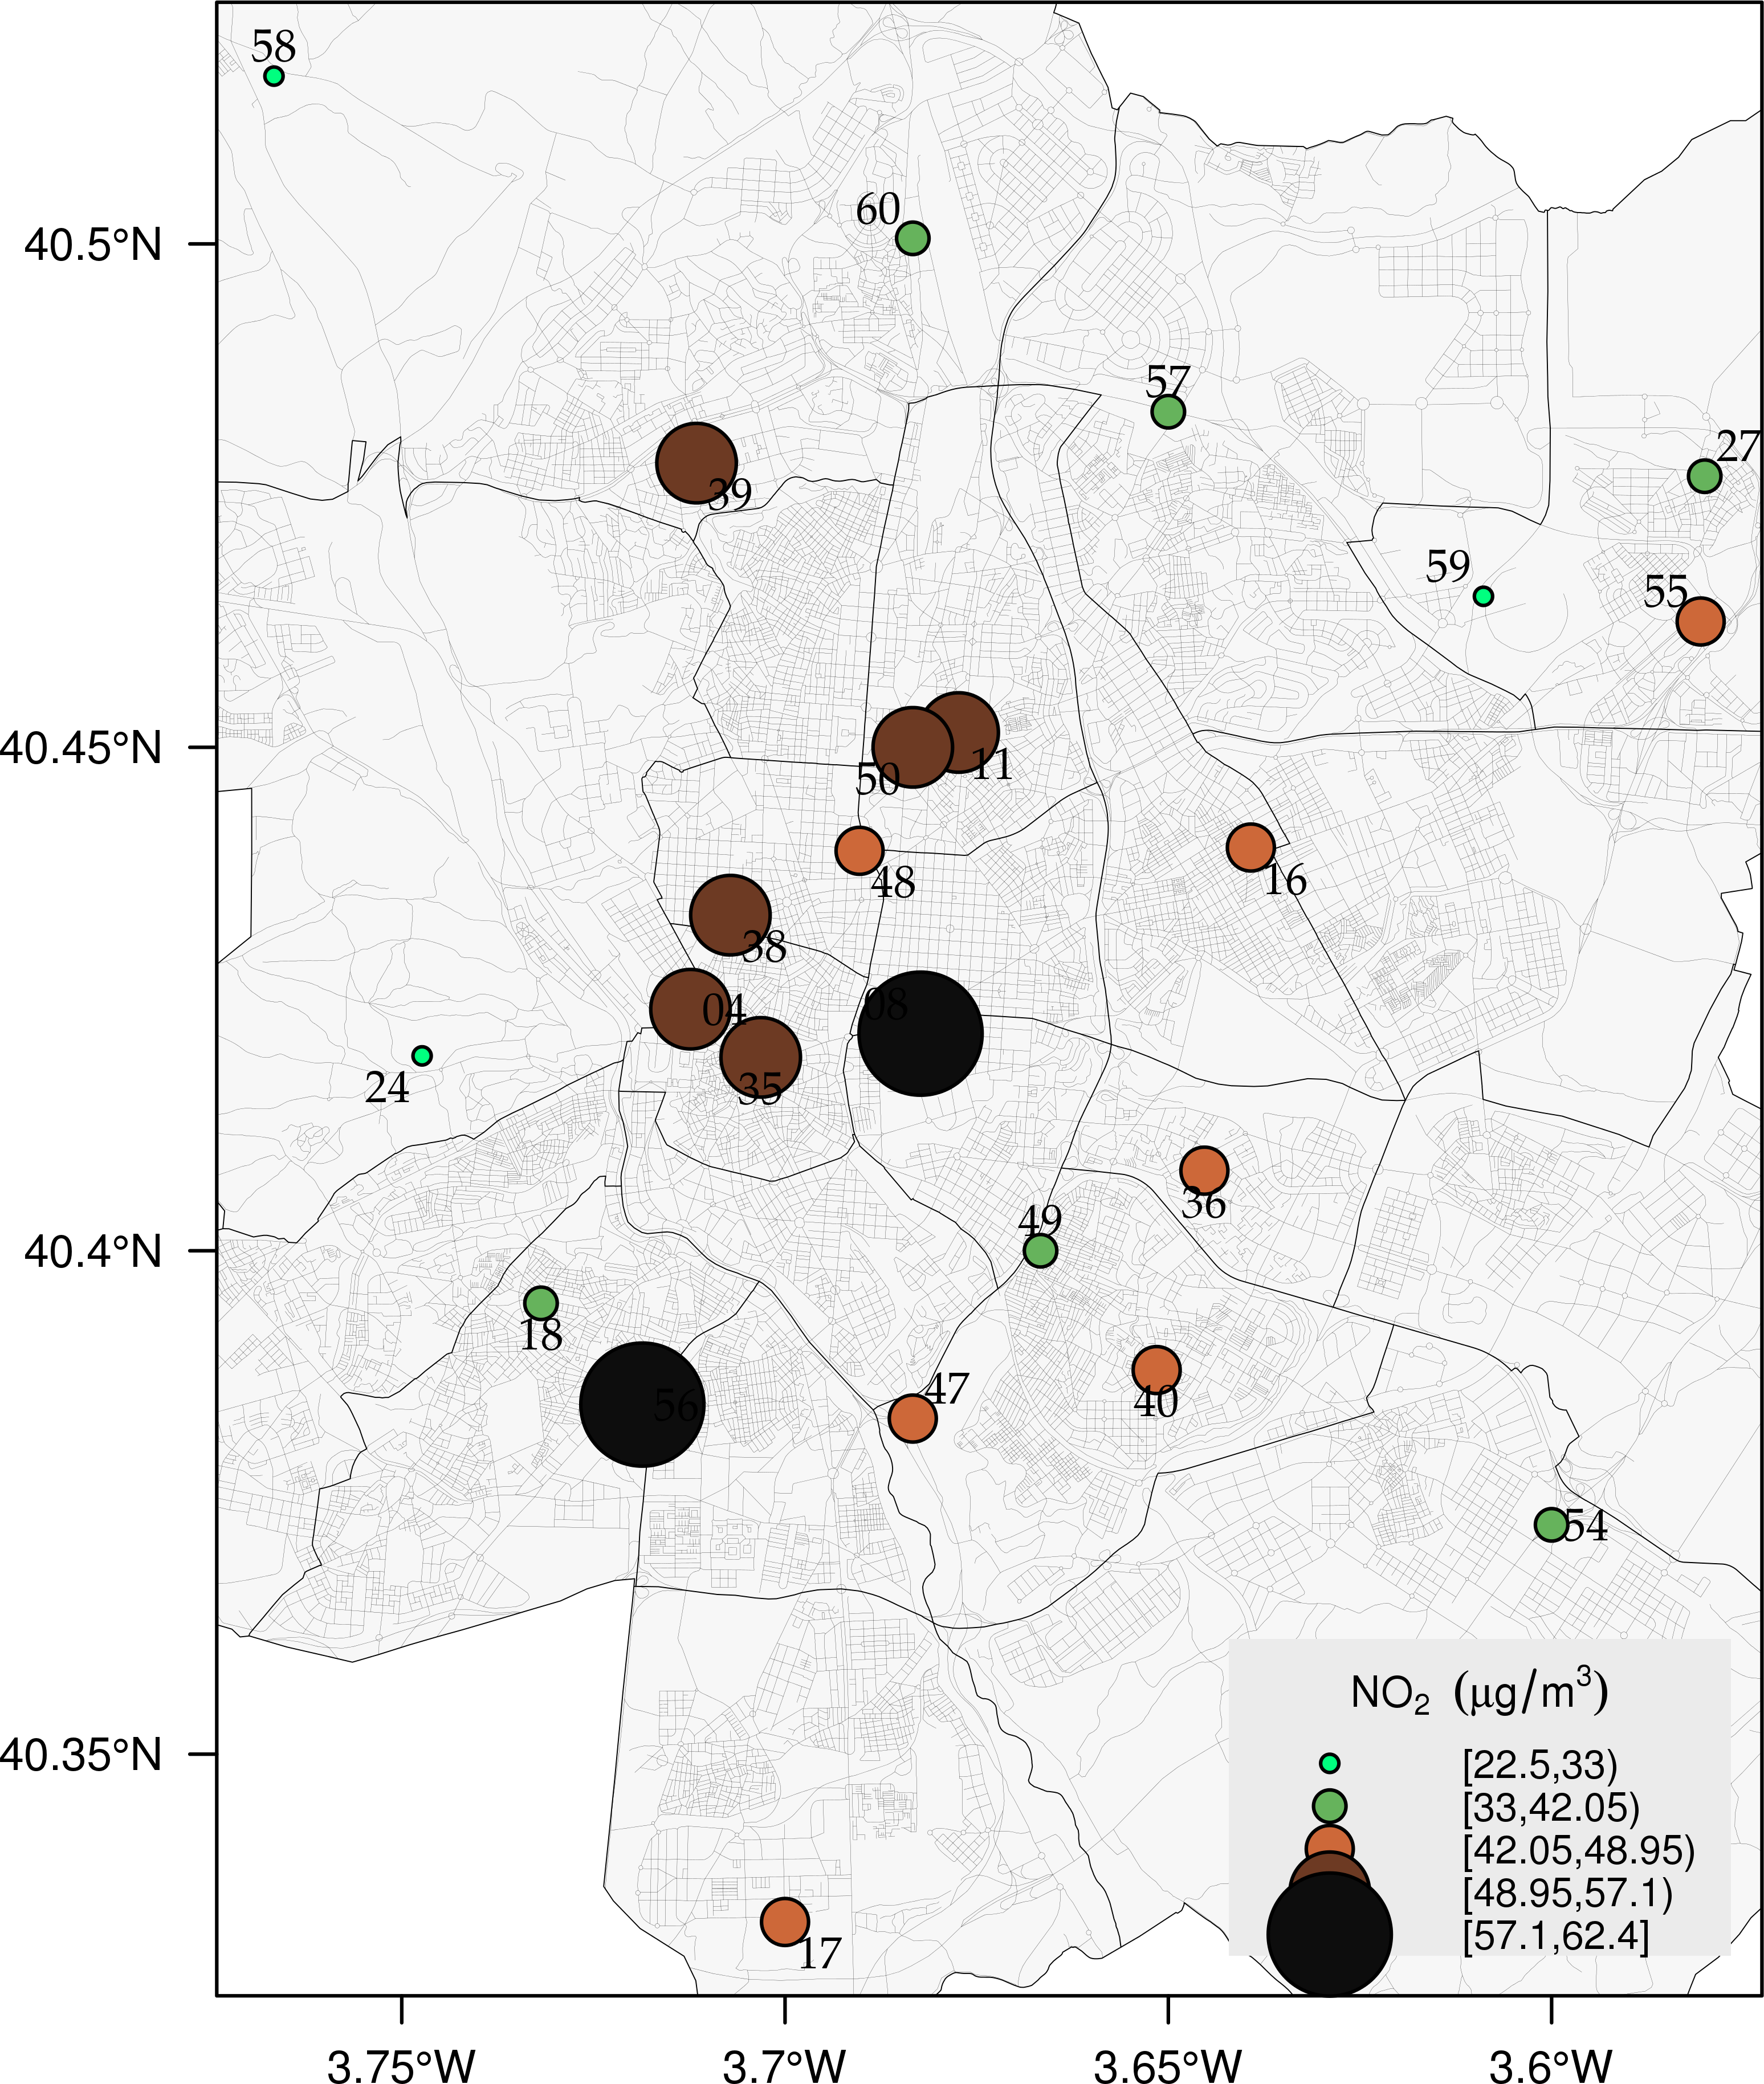
\includegraphics[width=.9\linewidth]{figs/airMadrid.png}
\caption{\label{fig:airMadrid}Annual average of $NO_2$ measurements in Madrid using shapefiles (lines and polygons) and text as geographical context.}
\end{figure}

The \texttt{ggplot2} package is not able to work directly with
\texttt{SpatialLines*} or \texttt{SpatialPolygon*} objects. Instead, it includes
several \texttt{fortify} methods to convert objects from these classes into a
conventional \texttt{data.frame}. You should beware that the \texttt{fortify}
process for large objects (such as the \texttt{SpatialLinesDataFrame} in our
example) requires too much time to be completed.

\subsection{Spatial Interpolation}
\label{sec-1-5}
The measurements at discrete points give limited information about the
underlying process. It is quite common to approximate the spatial
distribution of the measured variable with the interpolation between
measurement locations. Selection of the optimal interpolation method
is outside the scope of this book. The following code illustrates an
easy solution using inverse distance weighted (IDW) interpolation with
the \texttt{gstat} package \cite{Pebesma2004} \emph{only} for illustration
purposes.

\index{Packages!gstat@\texttt{gstat}}
\index{Packages!krige@\texttt{krige}}

\lstset{language=R,numbers=none}
\begin{lstlisting}
library(gstat)

airGrid <- spsample(NO2sp, type='regular', n=1e5)
gridded(airGrid) <- TRUE
airKrige <- krige(mean ~ 1, NO2sp, airGrid)
\end{lstlisting}

The result is a \texttt{SpatialPixelsDataFrame} that can be displayed with
\texttt{spplot} and combined with the previous layers and the measurement
station points (Figure \ref{fig:airMadrid_krige}).

\index{spplot@\texttt{spplot}}
\index{layer@\texttt{layer}}
\index{sp.polygons@\texttt{sp.polygons}}
\index{sp.lines@\texttt{sp.lines}}
\index{sp.points@\texttt{sp.points}}

\lstset{language=R,numbers=none}
\begin{lstlisting}
spplot(airKrige["var1.pred"],
       col.regions=colorRampPalette(airPal)) +
  layer({
    sp.polygons(distritosMadrid, fill='transparent', lwd=0.3)
    sp.lines(streetsMadrid, lwd=0.07)
    sp.points(NO2sp, pch=21, alpha=0.8, fill='gray50', col='black')
    })
\end{lstlisting}

\begin{figure}[htb]
\centering
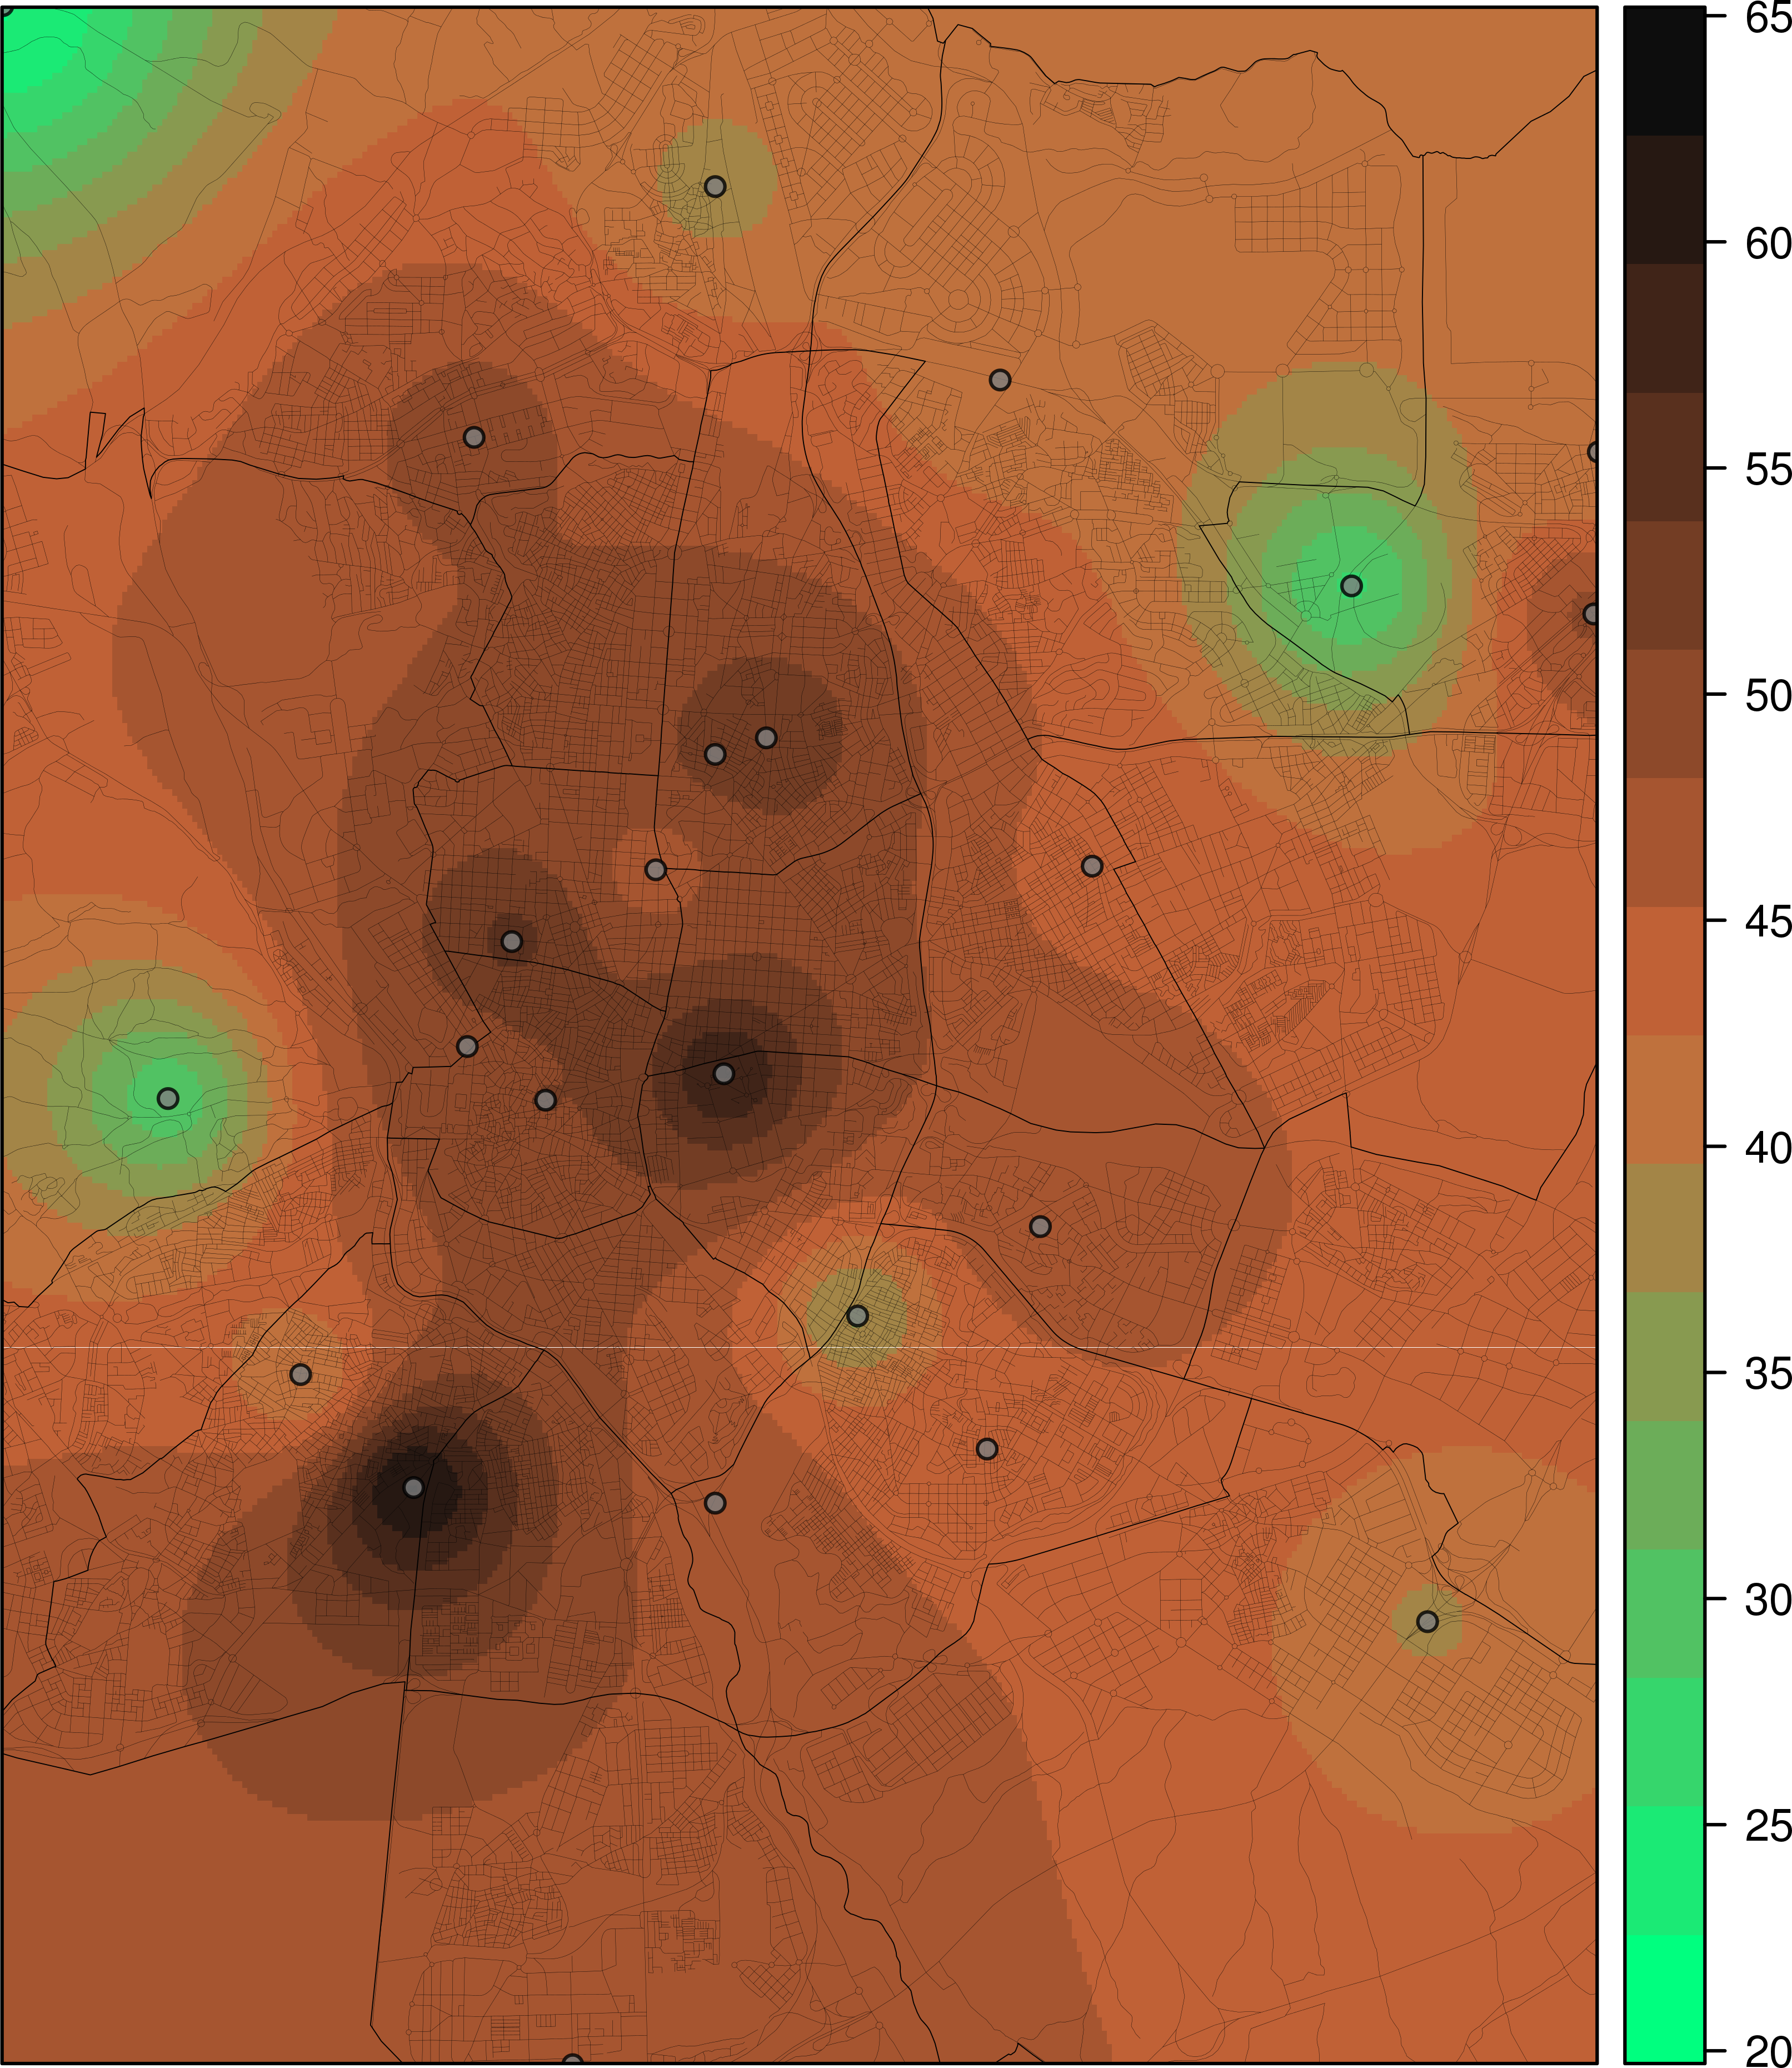
\includegraphics[width=.9\linewidth]{figs/airMadrid_krige.png}
\caption{\label{fig:airMadrid_krige}Kriging annual average of $NO_2$ measurements in Madrid.}
\end{figure}
\subsection{Export to Other Formats}
\label{sec-1-6}

A different approach is to use an external data viewer, due to its
features or its large community of users. Two tools deserve to be
mentioned: GeoJSON rendered within GitHub repositories, and KML files
imported in Google Earth\texttrademark.

\subsubsection{GeoJSON and OpenStreetMap}
\label{sec-1-6-1}
GeoJSON is an open computer file format for encoding collections of
simple geographical features along with their nonspatial attributes
using JavaScript Object Notation (JSON). These files can be easily
rendered within GitHub repositories. GitHub uses Leaflet.js\footnote{\url{http://leafletjs.com/}} to
represent the data and MapBox\footnote{\url{http://www.mapbox.com/}} with OpenStreetMap\footnote{\url{http://www.openstreetmap.org/}} for the
underlying map data.

Our \texttt{SpatialPointsDataFrame} can be converted to a GeoJSON file with
\texttt{writeOGR} from the \texttt{rgdal} package. 

\index{Packages!rgdal@\texttt{rgdal}}
\index{writeOGR@\texttt{writeOGR}}
\index{GeoJSON}

\lstset{language=R,numbers=none}
\begin{lstlisting}
library(rgdal)
writeOGR(NO2sp, 'data/NO2.geojson', 'NO2sp', driver='GeoJSON')
\end{lstlisting}

Figure \ref{fig:geojson} shows a snapshot of the rendering of this
GeoJSON file, available from the GitHub repository. There you can zoom
on the map and click on the stations to display the data.

\begin{figure}
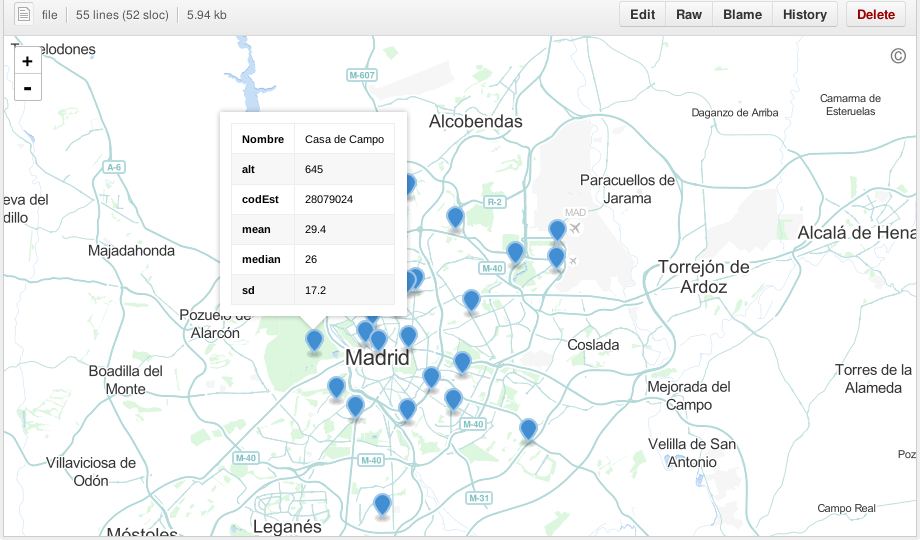
\includegraphics[width=0.9\textwidth]{figs/geojson.png}
\caption{\label{fig:geojson}$NO_2$ data in a GeoJSON file rendered within the GitHub repository.}
\end{figure}
\subsubsection{Keyhole Markup Language}
\label{sec-1-6-2}

Keyhole Markup Language (KML) is a file format to display geographic
data within Internet-based, two-dimensional maps and three-dimensional
Earth browsers. KML uses a tag-based structure with nested elements
and attributes, and is based on the XML standard. KML became an
international standard of the Open Geospatial Consortium
in 2008. Google Earth was the first program able to view and
graphically edit KML files, although Marble, an open-source project,
also offers KML support.

\index{Packages!rgdal@\texttt{rgdal}}
\index{Packages!plotKML@\texttt{plotKML}}
\index{KML}

There are several packages able to generate KML files. For example,
the \texttt{writeOGR} function from the \texttt{rgdal} package can also write KML
files:
\lstset{language=R,numbers=none}
\begin{lstlisting}
library(rgdal)
writeOGR(NO2sp, dsn='NO2_mean.kml', layer='mean', driver='KML')
\end{lstlisting}

However, the \texttt{plotKML} package provides a simpler interface and
includes a wide set of options:
\lstset{language=R,numbers=none}
\begin{lstlisting}
library(plotKML)
plotKML(NO2sp["mean"], points_names=NO2sp$codEst)
\end{lstlisting}

Both functions produce a file that can be directly opened with Google
Earth or Marble.
\subsection{\floweroneleft Additional Information with Tooltips and Hyperlinks}
\label{sec-1-7}
Now, let's suppose you need to know the median and standard deviation
of the time series of a certain station. Moreover, you would like to
watch the photography of that station; or even better, you wish to visit
its webpage for additional information. A frequent solution is to
produce interactive graphics with tooltips and hyperlinks.

The \texttt{gridSVG} package is able to create an SVG graphic, where each
component owns a \texttt{title} attribute; the content of this attribute is
commonly displayed as a tooltip when the mouse hovers over the
element. The content of this attribute can be modified thanks to the
\texttt{grid.garnish} function. Moreover, the \texttt{grid.hyperlink} function can
add hyperlinks to the correspondent graphical element.

The tooltips will display the photography of the station, the name of
the station, and the statistics previously calculated with \texttt{aggregate}
in the first step of this chapter.  The station images are downloaded
from the Munimadrid webpage. The \texttt{htmlParse} function from the \texttt{XML}
package parses each station page, and the station photograph is
extracted with \texttt{getNodeSet} and \texttt{xmlAttrs}.

\index{Packages!XML@\texttt{XML}}
\index{htmlParse@\texttt{htmlParse}}
\index{getNodeSet@\texttt{getNodeSet}}

\lstset{language=R,numbers=none}
\begin{lstlisting}
library(XML)

old <- setwd('images')
for (i in 1:nrow(NO2df)){
  codEst <- NO2df[i, "codEst"]
  ## Webpage of each station
  codURL <- as.numeric(substr(codEst, 7, 8))
  rootURL <- 'http://www.mambiente.munimadrid.es'
  stationURL <- paste(rootURL,
		      '/opencms/opencms/calaire/contenidos/estaciones/estacion',
		      codURL, '.html', sep='')
  content <- htmlParse(stationURL, encoding='utf8')
  ## Extracted with http://www.selectorgadget.com/
  xPath <- '//*[contains(concat( " ", @class, " " ), concat( " ", "imagen_1", " " ))]'
  imageStation <- getNodeSet(content, xPath)[[1]]
  imageURL <- xmlAttrs(imageStation)[1]
  imageURL <- paste(rootURL, imageURL, sep='')
  download.file(imageURL, destfile=paste(codEst, '.jpg', sep=''))
}
setwd(old)
\end{lstlisting}

Next, we attach the hyperlink and the SVG information to each
circle.


\index{Packages!gridSVG@\texttt{gridSVG}}
\index{JavaScript}
\index{grid.garnish@\texttt{grid.garnish}}
\index{grid.hyperlink@\texttt{grid.hyperlink}}
\index{grid.export@\texttt{grid.export}}

\lstset{language=R,numbers=none}
\begin{lstlisting}
print(pNO2 + layer_(sp.polygons(distritosMadrid, fill='gray97', lwd=0.3)))
\end{lstlisting}

\lstset{language=R,numbers=none}
\begin{lstlisting}
library(gridSVG)

NO2df <- as.data.frame(NO2sp)

tooltips <- sapply(seq_len(nrow(NO2df)), function(i){
  codEst <- NO2df[i, "codEst"]
  ## Information to be attached to each line
  stats <- paste(c('Mean', 'Median', 'SD'),
		 signif(NO2df[i, c('mean', 'median', 'sd')], 4),
		 sep=' = ', collapse='<br />')
  ## Station photograph 
  imageURL <- paste('images/', codEst, '.jpg', sep='')
  imageInfo <- paste("<img src=", imageURL,
		     " width='100' height='100' />", sep='')
  ## Text to be included in the tooltip
  nameStation <- paste('<b>', 
		       as.character(NO2df[i, "Nombre"]),
		       '</b>', sep='')
  info <- paste(nameStation, stats, sep='<br />')
  ## Tooltip includes the image and the text
  paste(imageInfo, info, sep='<br />')
})
grid.garnish('points.panel', title=tooltips,  grep=TRUE, group=FALSE)
\end{lstlisting}



\lstset{language=R,numbers=none}
\begin{lstlisting}
## Webpage of each station
rootURL <- 'http://www.mambiente.munimadrid.es'
urlList <- sapply(seq_len(nrow(NO2df)), function(i){
  codEst <- NO2df[i, "codEst"]
  codURL <- as.numeric(substr(codEst, 7, 8))
  stationURL <- paste(rootURL,
		      '/opencms/opencms/calaire/contenidos/estaciones/estacion',
		      codURL, '.html', sep='')
  })

grid.hyperlink('points.panel', urlList, grep=TRUE, group=FALSE)
\end{lstlisting}


The \texttt{title} attribute can be accessed with the JavaScript plug-ins
jQuery\footnote{\url{http://jquery.com/}} and jQuery UI\footnote{\url{http://jqueryui.com/}} to display tooltips when the mouse
hovers over each station. The \texttt{grid.script} function creates objects
containing links to these plug-ins. And \texttt{grid.export} uses these
objects to produce an SVG document with script elements.

\index{jQuery} 
\index{jQuery UI}

\lstset{language=R,numbers=none}
\begin{lstlisting}
## Add jQuery and jQuery UI scripts
grid.script(file='http://code.jquery.com/jquery-1.8.3.js')
grid.script(file='http://code.jquery.com/ui/1.9.2/jquery-ui.js')
## Simple JavaScript code to initialize the tooltip
grid.script(file='js/myTooltip.js')
## Produce the SVG graphic: the results of grid.garnish,
## grid.hyperlink and grid.script are converted to SVG code
grid.export('figs/airMadrid.svg')
\end{lstlisting}

These plug-ins will work only after the file \texttt{airMadrid.svg} created by
\texttt{grid.export} is inserted in a HTML file with standard headers. Figure
\ref{fig:airMadridTooltip} shows a capture of the result.

\lstset{language=R,numbers=none}
\begin{lstlisting}
htmlBegin <- '<!DOCTYPE html>
<html>
<head>
<title>Tooltips with jQuery and gridSVG</title>
<link rel="stylesheet" type="text/css" href="http://code.jquery.com/ui/1.9.2/themes/smoothness/jquery-ui.css" />
<meta charset="utf-8">
</head>
<body>'

htmlEnd <- '</body> </html>'

svgText <- paste(readLines('figs/airMadrid.svg'), collapse='\n')

writeLines(paste(htmlBegin, svgText, htmlEnd, sep='\n'),
	   'airMadrid.html')
\end{lstlisting}



\begin{figure}
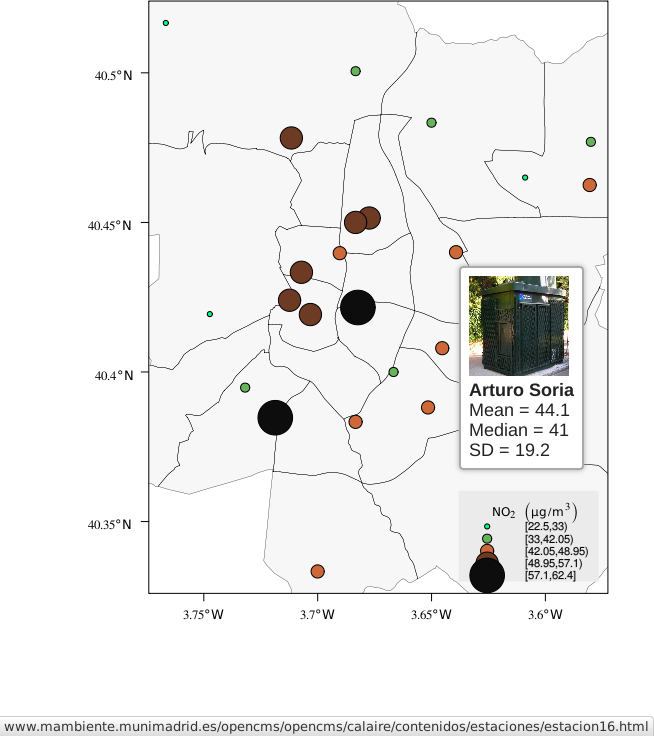
\includegraphics[width=0.9\textwidth]{figs/airMadridTooltip.png}
\caption{\label{fig:airMadridTooltip}Tooltips generated with \texttt{gridSVG} using jQuery and jQuery UI.}
\end{figure}
